\documentclass[../intro.tex]{subfiles}
\begin{document}

\section{Notation \& Definitions}

\begin{equation}
    A: \Gamma(E) \rightarrow \Gamma(H)
\end{equation}


 
\subsection{Data Space}
\begin{figure}[ht]
    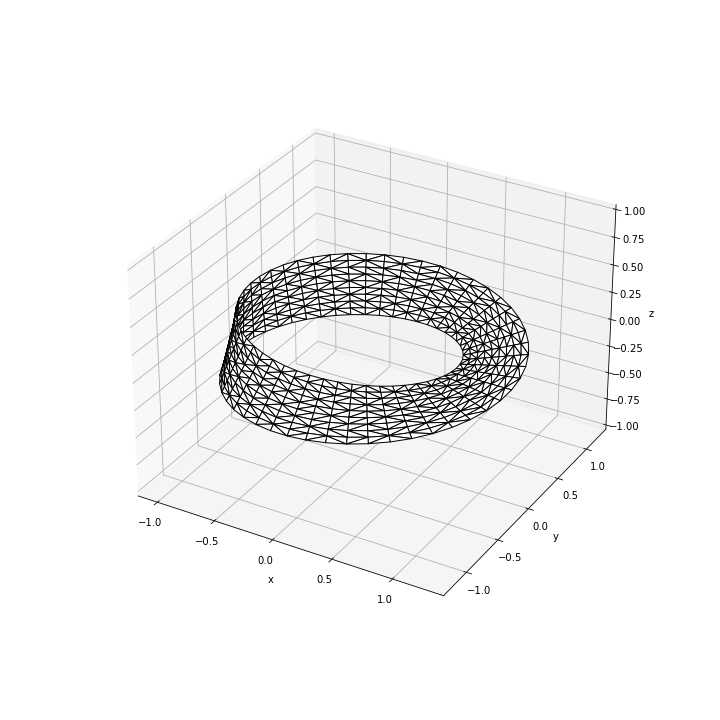
\includegraphics[width=0.5\linewidth]{figures/sections/math/mobius.png}
    \caption{write up some words here}
    \label{fig:mobius}
    %%possibly replace w/ simpler deconstructed band image notes-11-19-20
\end{figure}

We use a fiber bundle model to represent the data, as proposed by Butler 
\cite{butlerVectorBundleClassesForm1992,butlerVisualizationModelBased1989}. 


One example of a fiber bundle is the mobius band shown in figure~\ref{fig:mobius}. A fiber bundle is a topological total space $E$ with an embedded fiber space $F$, a base space on which the fibers lie $K$ and the $\pi$ and $\sigma$ mappings between $E$ and $K$. The space of all $\sigma$ is $\Gamma$ 

\begin{tikzcd}
    F \arrow[r, hook] & E \arrow[d, "\pi" description, bend right ] \\
                      & K \arrow[u, "\sigma" description, bend right]
\end{tikzcd}

As illustrated by the mobius band example in figure~\ref{fig:mobius}, the vertical lines $F$ are the range of possible values embedded in $E$. The circle $K$ is a representation of the connectivity of the points in $E$. The function $\pi$ is the mapping from a point on a specific fiber $F_{k}|k\in K$ in $E$ to a location $k \in K$.?  
The section $\sigma$ is the mapping from locations $k$ on $K$ to points on $F_{k}$ in $E$.  (Pull this back into more specific about fig, the general is making this more confusing.)

\subsubsection{Base Space $K$}

\begin{figure}[ht]
    \label{fig:simplex}
    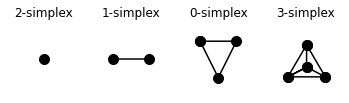
\includegraphics{figures/sections/math/simplex.png}
    \caption{Simplices encode the connectivity of the data, from fully disconnected (0 simplex) observations to all observations are connected to at least 3 other observations. Higher order simplicies are outside the scope of this paper.}
\end{figure}

One way to represent the topological space K is as a set composed of simplices, such as those shown in figure~\ref{fig:simplex}. Simplices are a way of encoding the connectivity of each observation ($\sigma(k)$) to another:

\begin{description}
    \item[0-simplex] discrete observations (inventory records)
    \item[1-simplex] 1D continuos data (timeseries)
    \item[2-simplex] 2D continuos data (map)
    \item[3-simplex] 3D continuos data (video)
\end{description}

In a locally trivial fiber bundle $E = F \times K$, it can be assumed that all $F_{k}$ for $k \in K$ are equal. A fiber bundle can be made locally trivial by approximating the total space E as a simplacial complex.

\subsubsection{Fiber Space $F$}
The fibers encode the set of all possible values each observation can take.  Spivak's formulation is that the fibers encode the union of the types of measurements\cite{spivakSIMPLICIALDATABASES}. For example, given the section $\Gamma(mobuis strip) =
\{\sigma_1=\sin, \sigma_2=\cos\}$:
%%fill in more spivak
the fiber $F = \{float, float\}$.  

%%% mapping from measurement back to type is the basis for gaurateening invariance 

\subsubsection{Subset \& Streaming}
$\Gamma(E)$ is the space of all points in $F$ returned by $\sigma$; therefore the points being visualized in a streaming or animation example can be considered a subset that lives on base space $U$ embedded in $K$ with the same fiber $\iota^*E$ and $\iota^*\sigma$.   

\begin{tikzcd}
    \iota^\ast E \arrow[r, hook] \arrow[d]                                                                       & E \arrow[d, bend right]                       \\
    U \arrow[r, "\iota" description, hook] \arrow[u, "\iota^\ast \sigma" description, bend right, shift right=2] & K \arrow[u, "\sigma" description, bend right]
\end{tikzcd}
%%% sheaves & presheaves 


\subsection{Display Space}
\label{sec:display}
\begin{figure}[h]
    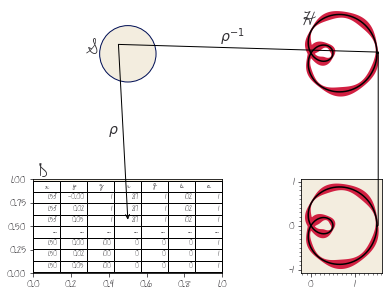
\includegraphics[width=.4\linewidth]{figures/sections/math/render.png}
    \caption{}
    \label{fig:render}
\end{figure}

A physical display space can be thought of sets of $\mathbb{R}^{7}$ tuples, where 
\begin{equation}
    \mathbb{R}^{7} = \{X, Y, Z, R, G, B, A\}
\end{equation}

and the sets correspond to the sections on $\S$, which is the topology of the output of the artist $A$. The space $H$ is a total space representing the predisplay space, with a fiber of $\mathbb{R}^7$ and a base space of $\S$:

\begin{tikzcd}
    \mathbb{R}^{7} \arrow[r, hook] & H \arrow[d, "\pi" description, bend right] \\
                                   & S \arrow[u, "\rho" description, bend right] 
\end{tikzcd}


In the case of 2D screens, the predisplay space is a trivial fiber bundle $H=\mathbb{R}^{7}\times S$. As illustrated in figure~\ref{fig:render}, a region on the screen defined by the corners $(x_1, y_1)$ and $(x_2, y_2)$ maps into a region on a 2-simplex in $S$ defined by $(\alpha_1, \beta_1)$ and $(\alpha_2, \beta_2)$. The function on the simplex $f$ returns the (R, G, B, A) value for that $(\alpha, \beta)$ pair. For a region, 

\begin{equation*}
\rho(S) = \int_{\alpha_1}^{\alpha_2}\int_{\beta_1}^{\beta_2}\int_{z_1}^{z_2}{R, G, B, A}  
\end{equation*}

where the R,G,B,A values are derived from the how the data values are mapped to visual characteristics. The z component of the mapping to $\mathbb{R}^7$ is moved to the integration because this is a trivial space representing a 2D screen; $\rho$ varies depending on $H$. 


\subsection{Artist}
\begin{equation}
    A: \Gamma(E) \rightarrow \Gamma(H)
\end{equation}

\subsubsection{Screen to Data}
%%diagram: [data] -Tau->[RGVXYZ]
%%%            \ /\ / 
\begin{tikzcd}
    E \arrow[d, "\pi" description] & H \arrow[d, "\pi" description]                                                 \\
    K \arrow[u, "\sigma" description, bend right] & S \arrow[l, "\xi" description] \arrow[u, "\rho" description, bend right]
\end{tikzcd}

The pullback $\xi$ on $S \rightarrow K$ means that the values in $E$ can be directly mapped to a simplex in $S$, which means there's a mapping from screen space back to the values. 

\begin{tikzcd}
    \xi E \arrow[rr, "\tau" description] \arrow[rd, "\xi \sigma" description, bend right] &     & H \arrow[ld] \\
    & S \arrow[lu, bend right] &             
\end{tikzcd}


\subsubsection{Marks}
%% diagram of connected components/line thing 11-19-20 notes
Bertin describes a location on the plane as the signifying characteristic of a point, measurable length as the signifying characteristic of a line, and measurable size as the signifying characteristic of an area and that in display (pixel) space these are marks \cite{bertinIIPropertiesGraphic2011,carpendaleVisualRepresentationSemiology}. 
\begin{equation}
\begin{tikzcd}
    H \arrow[r, shift left] & S \arrow[l, "\rho(\xi^{-1}(J))", shift left] \arrow[rr, "\xi(s)", shift left] &  & J_{k} =  \{j \in K| \exists \Gamma \text{ s.t. } \Gamma(0)=k \text{ and }\Gamma(1)=j\} \arrow[ll, "\xi^{-1}(J)", shift left]
\end{tikzcd}
\label{eq:mark}
\end{equation}

Each point $s$ in the display space $H$, the mark it belongs to can be found by mapping $s$ back to $K$ via the lookup on S described in section~\ref{sec:display} then taking $\xi(s)$ back to a point on $k \in K$ which lies on the connected component $J \subset K$. To got back to the display space $H$  from the simplacial complex $J$ of the signifier implanted in the mark, the inverse image of $J \in S, \xi^{-1}(J)$ is pushed back to $S$, and then  $\rho(\xi^{-1}(J))$ maps it into $R^{7}$. 



\subsubsection{Visual Characteristics}
Tau can preserves the measurement type properties (group scales)


\subsubsection{Visual Idioms: Equivalance class of artists}
Two artists are equivalent when given data containers $\Gamma(E)$ of the same type, they output the same type of prerender $\Gamma(S)$:
\begin{equation}
    \begin{tikzcd}
        A_{\tau_2}: \arrow[d, shift right=2] & \Gamma(E) \arrow[r] & \Gamma(H) &                                                \\
        A_{\tau_1}: \arrow[u, shift right]   & \Gamma(E) \arrow[r] & \Gamma(H) 
    \end{tikzcd}
\end{equation}

\end{document}